\documentclass[10pt]{article}% ===> this file was generated automatically by noweave --- better not edit it
\usepackage[a4paper, total={6in, 8in}]{geometry}
\usepackage{graphicx}
\graphicspath{ {./images/} }
\usepackage{noweb}
\usepackage{amsmath}
\usepackage{amssymb}
\usepackage{url}
\title{Extreme Learning Machine in J}
\author{Pierre-Edouard Portier}
\date{2019}
\renewcommand{\vec}[1]{\boldsymbol{#1}}
\newcommand{\norm}[1]{\left\lVert#1\right\rVert}

\begin{document}
\maketitle
\section{Regression}
$\vec{x^{(1)}}\dots\vec{x^{(P)}}$ are vectors of $\mathbb{R}^{n-1}$ with
associated values $y^{(1)}\dots y^{(P)}$ of $\mathbb{R}$.
We search a function $f(\vec{x}):\mathbb{R}^{n-1} \rightarrow \mathbb{R}$ to
model the observed relationship between $\vec{x}$ and $y$.
$f$ can have a fixed parameterized form. For example:
\[
f(\vec{x}) = a_0 + a_1 x_1 + a_2 x_2 + \dots + a_{n-1} x_{n-1}
\]

If $P=n$, parameters $a_0 \dots a_{n-1}$ are found by solving a linear system.
\[
\begin{cases}
y^{(1)} &= a_0 + a_1 x_1^{(1)} + a_2 x_2^{(1)} + \dots + a_{n-1} x_{n-1}^{(1)} \\
\dots &= \dots \\
y^{(P)} &= a_0 + a_1 x_1^{(P)} + a_2 x_2^{(P)} + \dots + a_{n-1} x_{n-1}^{(P)} \\
\end{cases}
\]
This system can be written In matrix form.
\[
\left( \begin{array}{cccc}
1 & x^{(1)}_1 & \dots & x^{(1)}_{n-1} \\
1 & x^{(2)}_1 & \dots & x^{(2)}_{n-1} \\
\dots & \dots & \dots & \dots \\
1 & x^{(P)}_1 & \dots & x^{(P)}_{n-1}
\end{array} \right)
\left( \begin{array}{c}
a_0 \\ a_1 \\ \dots \\ a_{n-1} 
\end{array} \right)
=
\left( \begin{array}{c}
y^{(1)} \\ y^{(2)} \\ \dots \\ y^{(P)} 
\end{array} \right)
\]

Each line of the first term matrix is a vector $\vec{x^{(i)T}}$ with the
addition of a constant coordinate that accounts for parameter $a_0$.
Thus, naming this matrix $\vec{X}^T$, the linear system can also be written:
\[
\vec{X}^T \vec{a} = \vec{y}
\]

Consider the special case when $x$ is a number and $f$ is a polynomial of degree $n-1$:
\[
f(x) = a_0 + a_1 x + a_2 x^2 + \dots + a_{n-1}x^{n-1}
\]

With $P=n$ examples $\left(x^{(k)},y^{(k)}\right)$, the parameters are found by
solving the following linear system:
\begin{equation}
\left( \begin{array}{ccccc}
1 & x^{(1)} & (x^{(1)})^2 & \dots & (x^{(1)})^{n-1} \\
1 & x^{(2)} & (x^{(2)})^2 & \dots & (x^{(2)})^{n-1} \\
\dots & \dots & \dots & \dots \\
1 & x^{(P)} & (x^{(P)})^2 & \dots & (x^{(P)})^{n-1}
\end{array} \right)
\left( \begin{array}{c}
a_0 \\ a_1 \\ \dots \\ a_{n-1} 
\end{array} \right)
=
\left( \begin{array}{c}
y^{(1)} \\ y^{(2)} \\ \dots \\ y^{(P)} 
\end{array} \right)
\label{eqn:vandermonde}
\end{equation}
Incidentally, the first term is called the Vandermonde Matrix.

\subsection{Experiment with a 1-dimensional synthetic dataset}
We define a non linear function {\Tt{}f\nwendquote} from which we generate a dataset

\nwfilename{jelm.nw}\nwbegincode{1}\sublabel{NWS2xmL-1BDS9S-1}\nwmargintag{{\nwtagstyle{}\subpageref{NWS2xmL-1BDS9S-1}}}\moddef{dataset~{\nwtagstyle{}\subpageref{NWS2xmL-1BDS9S-1}}}\endmoddef\nwstartdeflinemarkup\nwusesondefline{\\{NWS2xmL-2IxhEH-1}}\nwenddeflinemarkup
f=: 3 : '(^y) * cos 2*pi * sin pi * y'
\LA{}noise~{\nwtagstyle{}\subpageref{NWS2xmL-148nWG-1}}\RA{}
\LA{}gendat~{\nwtagstyle{}\subpageref{NWS2xmL-15el3j-1}}\RA{}

\nwused{\\{NWS2xmL-2IxhEH-1}}\nwendcode{}\nwbegindocs{2}\nwdocspar
In traditional mathematical form, this function is: 
\[f(x)=e^x \times cos\left(2\pi sin\left(\pi x\right)\right)\]

Function {\Tt{}noise\nwendquote} adds some random noise to the values of a vector. For
example {\Tt{}0.5\ noise\ v\nwendquote}, will add random values uniformly drawn from interval
$[-0.5,0.5]$ to the terms of vector {\Tt{}v\nwendquote}.

\nwenddocs{}\nwbegincode{3}\sublabel{NWS2xmL-148nWG-1}\nwmargintag{{\nwtagstyle{}\subpageref{NWS2xmL-148nWG-1}}}\moddef{noise~{\nwtagstyle{}\subpageref{NWS2xmL-148nWG-1}}}\endmoddef\nwstartdeflinemarkup\nwusesondefline{\\{NWS2xmL-1BDS9S-1}}\nwenddeflinemarkup
noise=: 4 : 'y + -&x *&(+:x) ? (#y) # 0'

\nwused{\\{NWS2xmL-1BDS9S-1}}\nwendcode{}\nwbegindocs{4}\nwdocspar
{\Tt{}0.5\ gendat\ 10\nwendquote} generates from {\Tt{}f\nwendquote} a dataset {\Tt{}(X,Y)\nwendquote} of 10 points with
random noise in $[-0.5,0.5]$ added to {\Tt{}Y\nwendquote}. It also stores in {\Tt{}minmaxX\nwendquote} the
minimum and maximum values of {\Tt{}X\nwendquote}. It computes the pair {\Tt{}minmaxf\nwendquote},
where the first term is ten percent smaller than the minimum of {\Tt{}f\nwendquote} on interval
$[0,1]$, and the second term is ten percent bigger than the maximum of {\Tt{}f\nwendquote} on
interval $[0,1]$. {\Tt{}minmaxf\nwendquote} is later used to crop the plots so that
extreme values are not visible.

\nwenddocs{}\nwbegincode{5}\sublabel{NWS2xmL-qrUr4-1}\nwmargintag{{\nwtagstyle{}\subpageref{NWS2xmL-qrUr4-1}}}\moddef{utils~{\nwtagstyle{}\subpageref{NWS2xmL-qrUr4-1}}}\endmoddef\nwstartdeflinemarkup\nwusesondefline{\\{NWS2xmL-2IxhEH-1}}\nwprevnextdefs{\relax}{NWS2xmL-qrUr4-2}\nwenddeflinemarkup
pushup=:   ] + 0.1 * |
pushdown=: ] - 0.1 * |

\nwalsodefined{\\{NWS2xmL-qrUr4-2}\\{NWS2xmL-qrUr4-3}\\{NWS2xmL-qrUr4-4}\\{NWS2xmL-qrUr4-5}}\nwused{\\{NWS2xmL-2IxhEH-1}}\nwendcode{}\nwbegincode{6}\sublabel{NWS2xmL-15el3j-1}\nwmargintag{{\nwtagstyle{}\subpageref{NWS2xmL-15el3j-1}}}\moddef{gendat~{\nwtagstyle{}\subpageref{NWS2xmL-15el3j-1}}}\endmoddef\nwstartdeflinemarkup\nwusesondefline{\\{NWS2xmL-1BDS9S-1}}\nwenddeflinemarkup
gendat=: 4 : 0
  X=: ? y $ 0
  Y=: x noise f X
  minmaxX=: (<./ , >./) X
  minmaxf=: (([: pushdown <./) , ([: pushup >./)) f steps 0 1 100
  \LA{}testdat~{\nwtagstyle{}\subpageref{NWS2xmL-15TB7-1}}\RA{}
)

\nwused{\\{NWS2xmL-1BDS9S-1}}\nwendcode{}\nwbegindocs{7}\nwdocspar
{\Tt{}plotdat\ 0\nwendquote} plots the dataset.

\nwenddocs{}\nwbegincode{8}\sublabel{NWS2xmL-MlnJE-1}\nwmargintag{{\nwtagstyle{}\subpageref{NWS2xmL-MlnJE-1}}}\moddef{plotdat~{\nwtagstyle{}\subpageref{NWS2xmL-MlnJE-1}}}\endmoddef\nwstartdeflinemarkup\nwusesondefline{\\{NWS2xmL-2IxhEH-1}}\nwenddeflinemarkup
plotdatnoshow=: 3 : 0
  \LA{}initplot~{\nwtagstyle{}\subpageref{NWS2xmL-1JSNQW-1}}\RA{}
  pd X;Y
  \LA{}plotf~{\nwtagstyle{}\subpageref{NWS2xmL-4gTINf-1}}\RA{}
)
plotdat=: 3 : 0
  plotdatnoshow 0
  pd 'show'
)

\nwused{\\{NWS2xmL-2IxhEH-1}}\nwendcode{}\nwbegincode{9}\sublabel{NWS2xmL-1JSNQW-1}\nwmargintag{{\nwtagstyle{}\subpageref{NWS2xmL-1JSNQW-1}}}\moddef{initplot~{\nwtagstyle{}\subpageref{NWS2xmL-1JSNQW-1}}}\endmoddef\nwstartdeflinemarkup\nwusesondefline{\\{NWS2xmL-MlnJE-1}\\{NWS2xmL-D6YgQ-1}}\nwenddeflinemarkup
pd 'reset'
pd 'color green'
pd 'type marker'
pd 'markersize 1'
pd 'markers circle'

\nwused{\\{NWS2xmL-MlnJE-1}\\{NWS2xmL-D6YgQ-1}}\nwendcode{}\nwbegincode{10}\sublabel{NWS2xmL-4gTINf-1}\nwmargintag{{\nwtagstyle{}\subpageref{NWS2xmL-4gTINf-1}}}\moddef{plotf~{\nwtagstyle{}\subpageref{NWS2xmL-4gTINf-1}}}\endmoddef\nwstartdeflinemarkup\nwusesondefline{\\{NWS2xmL-MlnJE-1}\\{NWS2xmL-D6YgQ-1}}\nwenddeflinemarkup
pd 'color red'
pd 'type line'
pd 'pensize 1'
pd (;f) steps 0 1 100

\nwused{\\{NWS2xmL-MlnJE-1}\\{NWS2xmL-D6YgQ-1}}\nwendcode{}\nwbegindocs{11}\nwdocspar
\noindent\begin{minipage}{0.5\textwidth}
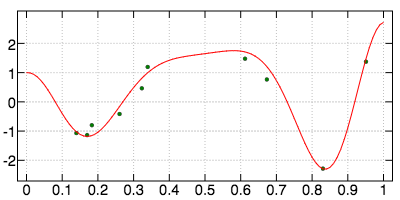
\includegraphics[width=\linewidth]{plotdat}
\end{minipage}%
\hfill%
\begin{minipage}{0.4\textwidth}
\begin{verbatim}
   0.5 gendat 10
_2.53128 2.99011
   plotdat 0
\end{verbatim}
\end{minipage}
\vskip.5\baselineskip

{\Tt{}polyreg\ 0\nwendquote} solves the linear system \eqref{eqn:vandermonde} and stores the
coefficients of the polynomial in variable {\Tt{}c\nwendquote}.

\nwenddocs{}\nwbegincode{12}\sublabel{NWS2xmL-16Ud8S-1}\nwmargintag{{\nwtagstyle{}\subpageref{NWS2xmL-16Ud8S-1}}}\moddef{polyreg~{\nwtagstyle{}\subpageref{NWS2xmL-16Ud8S-1}}}\endmoddef\nwstartdeflinemarkup\nwusesondefline{\\{NWS2xmL-2IxhEH-1}}\nwenddeflinemarkup
polyreg=: 3 : 0
  c=: Y ([ %. ] ^/ i.@#@]) X
  plotpoly 0
)

\nwused{\\{NWS2xmL-2IxhEH-1}}\nwendcode{}\nwbegincode{13}\sublabel{NWS2xmL-qrUr4-2}\nwmargintag{{\nwtagstyle{}\subpageref{NWS2xmL-qrUr4-2}}}\moddef{utils~{\nwtagstyle{}\subpageref{NWS2xmL-qrUr4-1}}}\plusendmoddef\nwstartdeflinemarkup\nwusesondefline{\\{NWS2xmL-2IxhEH-1}}\nwprevnextdefs{NWS2xmL-qrUr4-1}{NWS2xmL-qrUr4-3}\nwenddeflinemarkup
NB. identify the elements with values between \{.x and \{:x
sel=: (] >: \{.@[) *. (] <: \{:@[)

\nwused{\\{NWS2xmL-2IxhEH-1}}\nwendcode{}\nwbegincode{14}\sublabel{NWS2xmL-44Bx4d-1}\nwmargintag{{\nwtagstyle{}\subpageref{NWS2xmL-44Bx4d-1}}}\moddef{plotpoly~{\nwtagstyle{}\subpageref{NWS2xmL-44Bx4d-1}}}\endmoddef\nwstartdeflinemarkup\nwusesondefline{\\{NWS2xmL-2IxhEH-1}}\nwenddeflinemarkup
plotpoly=: 3 : 0
  plotdatnoshow 0
  pd 'color blue'
  xs=: (] #~ minmaxX"_ sel ]) /:~ X,steps 0 1 100
  pval=: c&p. xs
  crop=: minmaxf sel pval
  pd (crop # xs);(crop # pval)
  pd 'show'
)

\nwused{\\{NWS2xmL-2IxhEH-1}}\nwendcode{}\nwbegindocs{15}\nwdocspar
\noindent\begin{minipage}{0.5\textwidth}
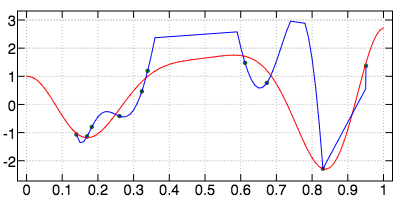
\includegraphics[width=\linewidth]{polyreg}
\end{minipage}%
\hfill%
\begin{minipage}{0.4\textwidth}
\begin{verbatim}
   polyreg 0
\end{verbatim}
\end{minipage}
\vskip.5\baselineskip

\subsection{Generalization to a function space}
Given a basis for a function space, we can try to express {\Tt{}f\nwendquote} as a combination
of basis functions.
\[
f(\vec{x}) = a_1 f_1(\vec{x}) + a_2 f_2(\vec{x}) + \dots + a_n f_n(\vec{x})
\]

Given a dataset of $n$ pairs $\biggl(\vec{x}^{(k)},\vec{y}^{(k)}\biggr)$, the
coefficients $a_i$ are found by solving a linear system.

\[
\left( \begin{array}{ccccc}
f_1(\vec{x}^{(1)}) & f_2(\vec{x}^{(1)}) & \dots & f_n(\vec{x}^{(1)}) \\
f_1(\vec{x}^{(2)}) & f_2(\vec{x}^{(2)}) & \dots & f_n(\vec{x}^{(2)}) \\
\dots & \dots & \dots & \dots \\
f_1(\vec{x}^{(n)}) & f_2(\vec{x}^{(n)}) & \dots & f_n(\vec{x}^{(n)})
\end{array} \right)
\left( \begin{array}{c}
a_1 \\ a_2 \\ \dots \\ a_{n} 
\end{array} \right)
=
\left( \begin{array}{c}
y^{(1)} \\ y^{(2)} \\ \dots \\ y^{(n)} 
\end{array} \right)
\]

Let us denote this linear system by $\vec{A}\vec{x}=\vec{b}$.

\subsection{Least squares}
With more examples than the number of basis functions, the linear system
$\vec{A}\vec{x}=\vec{b}$ (with $\vec{A} \in \mathbb{R}^{m \times n}$) doesn't
necessarily have a solution.
Thus, we want to find an approximate solution $\vec{A}\vec{x}\approx\vec{b}$
that minimizes the squares of the errors: $\norm{\vec{A}\vec{x}-\vec{b}}^2_2$.

\begin{align*}
 & \norm{\vec{A}\vec{x}-\vec{b}}^2_2 \\
= \{ & \norm{\vec{x}}_2 = \sqrt{\vec{x}\cdot\vec{x}} \} \\
 & \left(\vec{A}\vec{x}-\vec{b}\right) \cdot \left(\vec{A}\vec{x}-\vec{b}\right) \\
= \{ & \text{euclidean scalar product} \} \\
 & \left(\vec{A}\vec{x}-\vec{b}\right)^T \left(\vec{A}\vec{x}-\vec{b}\right) \\
= \{ & \text{property of transposition} \} \\
 & \left(\vec{x}^T\vec{A}^T - \vec{b}^T \right) \left(\vec{A}\vec{x}-\vec{b}\right) \\
= \{ & \text{multiplication} \} \\
 & \vec{x}^T\vec{A}^T\vec{A}\vec{x} - \vec{x}^T\vec{A}^T\vec{b} - \vec{b}^T\vec{A}\vec{x} + \vec{b}^T\vec{b} \\
= \{ & \text{Since each element of the sum is a scalar, } \vec{b}^T\vec{A}\vec{x} = \left(\vec{b}^T\vec{A}\vec{x}\right)^T = \vec{x}^T\vec{A}^T\vec{b} \} \\
 & \vec{x}^T\vec{A}^T\vec{A}\vec{x} - 2\vec{x}^T\vec{A}^T\vec{b} + \vec{b}^T\vec{b}
\end{align*}

To this quadratic expression corresponds a convex surface.
Its minimum is found by setting the derivative to zero.

\begin{align*}
 & \vec{0} = 2\vec{A}^T\vec{A}\vec{x} - 2\vec{A}^T\vec{b} \\
=& \\
 & \vec{A}^T\vec{A}\vec{x} = \vec{A}^T\vec{b}
\end{align*}

Thus, when $m>n$, we solve $\vec{A}\vec{x}\approx\vec{b}$ by solving
$\vec{A}^T\vec{A}\vec{x} = \vec{A}^T\vec{b}$.
$\vec{A}^T\vec{A}$ is called the Gram matrix.

{\Tt{}gram\ y\nwendquote} computes the Gram matrix {\Tt{}S\nwendquote} for a polynomial basis of degree {\Tt{}y-1\nwendquote}.

\nwenddocs{}\nwbegincode{16}\sublabel{NWS2xmL-4YHogE-1}\nwmargintag{{\nwtagstyle{}\subpageref{NWS2xmL-4YHogE-1}}}\moddef{gram~{\nwtagstyle{}\subpageref{NWS2xmL-4YHogE-1}}}\endmoddef\nwstartdeflinemarkup\nwusesondefline{\\{NWS2xmL-2IxhEH-1}}\nwprevnextdefs{\relax}{NWS2xmL-4YHogE-2}\nwenddeflinemarkup
gram=: 3 : 0
  A=: X ^/ i.y
  S=: (mp~ |:) A
) 

\nwalsodefined{\\{NWS2xmL-4YHogE-2}}\nwused{\\{NWS2xmL-2IxhEH-1}}\nwendcode{}\nwbegincode{17}\sublabel{NWS2xmL-qrUr4-3}\nwmargintag{{\nwtagstyle{}\subpageref{NWS2xmL-qrUr4-3}}}\moddef{utils~{\nwtagstyle{}\subpageref{NWS2xmL-qrUr4-1}}}\plusendmoddef\nwstartdeflinemarkup\nwusesondefline{\\{NWS2xmL-2IxhEH-1}}\nwprevnextdefs{NWS2xmL-qrUr4-2}{NWS2xmL-qrUr4-4}\nwenddeflinemarkup
mp=: +/ . * NB. matrix product

\nwused{\\{NWS2xmL-2IxhEH-1}}\nwendcode{}\nwbegindocs{18}\nwdocspar

{\Tt{}leastsq\ y\nwendquote} solves the overdetermined linear system by computing the Gram
matrix for a polynomial basis of degree {\Tt{}y-1\nwendquote}.

\nwenddocs{}\nwbegincode{19}\sublabel{NWS2xmL-4YHogE-2}\nwmargintag{{\nwtagstyle{}\subpageref{NWS2xmL-4YHogE-2}}}\moddef{gram~{\nwtagstyle{}\subpageref{NWS2xmL-4YHogE-1}}}\plusendmoddef\nwstartdeflinemarkup\nwusesondefline{\\{NWS2xmL-2IxhEH-1}}\nwprevnextdefs{NWS2xmL-4YHogE-1}{\relax}\nwenddeflinemarkup
leastsq=: 3 : 0
  gram y
  c=: ((|:A) mp Y) %. S
  plotpoly 0
)

\nwused{\\{NWS2xmL-2IxhEH-1}}\nwendcode{}\nwbegindocs{20}\nwdocspar
\noindent\begin{minipage}{0.5\textwidth}
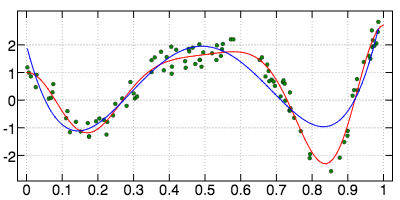
\includegraphics[width=\linewidth]{leastsq5}
\end{minipage}%
\hfill%
\begin{minipage}{0.4\textwidth}
\begin{verbatim}
   0.5 gendat 100
_2.53128 2.99011
   leastsq 5
\end{verbatim}
\end{minipage}

\noindent\begin{minipage}{0.5\textwidth}
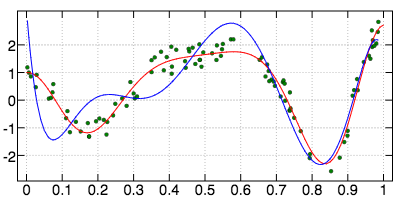
\includegraphics[width=\linewidth]{leastsq8}
\end{minipage}%
\hfill%
\begin{minipage}{0.4\textwidth}
\begin{verbatim}
   leastsq 8
\end{verbatim}
\end{minipage}
\vskip.5\baselineskip

\subsection{Tikhonov regularization}
With less examples than the number of basis functions (i.e. $m<n$,
underdetermined system), $\vec{A}\vec{x}=\vec{b}$ doesn't have a unique solution.
Even with $m\geq n$, the linear system can have approximate solutions more
desirable than the optimal one. In particular, this is the case when several
examples are very similar. For example, the solution to\dots

\[
\left( \begin{array}{cc}
1 & 1 \\
1 & 1.00001 \\
\end{array} \right)
\left( \begin{array}{c}
x_1 \\ x_2
\end{array} \right)
=
\left( \begin{array}{c}
1 \\ 0.99 
\end{array} \right)
\]

\dots is $\vec{x}^T = (1001,-1000)$. However, the approximate solution
$\vec{x}^T = (0.5,0.5)$ is  more suitable. Indeed, the optimal solution is not
likely to adapt well to new inputs (e.g., input $(1,2)$ would be projected onto
$-999$\dots).

Thus, when several solutions are feasible, we want to favor smaller
norms $\norm{x}_2$ by solving a new minimization problem:

\begin{align*}
\min_{\vec{x}} \norm{\vec{A}\vec{x}-\vec{b}}^2_2 + \alpha \norm{\vec{x}}^2_2 \\
with \quad 0 < \alpha < 1
\end{align*}

The minimum of this expression is found by setting its derivative to zero.

\begin{align*}
 & \vec{0} = 2\vec{A}^T\vec{A}\vec{x} - 2\vec{A}^T\vec{b} + 2\alpha\vec{x} \\
=& \\
 & \left( \vec{A}^T\vec{A} + \alpha \vec{I}_{n\times n} \right) \vec{x} = \vec{A}^T \vec{b}
\end{align*}

It comes down to adding a small positive value to the diagonal of the
Gram matrix. This approach has been given several names: Tikhonov regularization,
ridge regression\dots

{\Tt{}1E{\_}3\ ridge\ 5\nwendquote} will solve the ridge regression for a polynomial basis of
degree $5$ and a regularization coefficient equal to $10^{-3}$.

\nwenddocs{}\nwbegincode{21}\sublabel{NWS2xmL-Vqgr5-1}\nwmargintag{{\nwtagstyle{}\subpageref{NWS2xmL-Vqgr5-1}}}\moddef{ridge~{\nwtagstyle{}\subpageref{NWS2xmL-Vqgr5-1}}}\endmoddef\nwstartdeflinemarkup\nwusesondefline{\\{NWS2xmL-2IxhEH-1}}\nwenddeflinemarkup
ridge=: 4 : 0
  gram y
  c=: ((|:A) mp Y) %.  x addDiag S
  plotpoly 0
)

\nwused{\\{NWS2xmL-2IxhEH-1}}\nwendcode{}\nwbegincode{22}\sublabel{NWS2xmL-qrUr4-4}\nwmargintag{{\nwtagstyle{}\subpageref{NWS2xmL-qrUr4-4}}}\moddef{utils~{\nwtagstyle{}\subpageref{NWS2xmL-qrUr4-1}}}\plusendmoddef\nwstartdeflinemarkup\nwusesondefline{\\{NWS2xmL-2IxhEH-1}}\nwprevnextdefs{NWS2xmL-qrUr4-3}{NWS2xmL-qrUr4-5}\nwenddeflinemarkup
diag=: (<0 1)&|: : (([:(>:*i.)[:#])\})
addDiag=: ([+diag@]) diag ] NB. add x to the diagonal of y

\nwused{\\{NWS2xmL-2IxhEH-1}}\nwendcode{}\nwbegindocs{23}\nwdocspar
\noindent\begin{minipage}{0.5\textwidth}
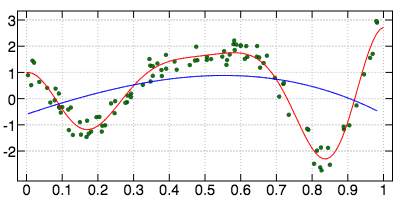
\includegraphics[width=\linewidth]{ridge4}
\end{minipage}%
\hfill%
\begin{minipage}{0.4\textwidth}
\begin{verbatim}
   1E_4 ridge 4
\end{verbatim}
\end{minipage}
\vskip.5\baselineskip

\noindent\begin{minipage}{0.5\textwidth}
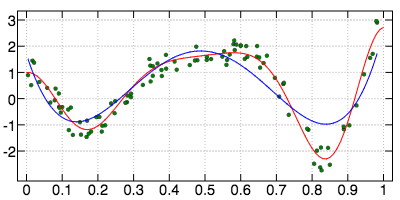
\includegraphics[width=\linewidth]{ridge5}
\end{minipage}%
\hfill%
\begin{minipage}{0.4\textwidth}
\begin{verbatim}
   1E_4 ridge 5
\end{verbatim}
\end{minipage}
\vskip.5\baselineskip

\noindent\begin{minipage}{0.5\textwidth}
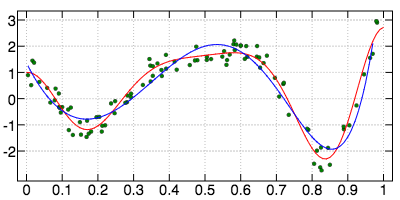
\includegraphics[width=\linewidth]{ridge8}
\end{minipage}%
\hfill%
\begin{minipage}{0.4\textwidth}
\begin{verbatim}
   1E_4 ridge 8
\end{verbatim}
\end{minipage}
\vskip.5\baselineskip

\subsection{Extreme Learning Machine}
The following parametrized form of $f$ corresponds to a single hidden layer
neural network.
\[
f(\vec{x}) = c_1 g(\vec{w_1}\cdot\vec{x}+b_1) + c_2 g(\vec{w_2}\cdot\vec{x}+b_2) 
+ \dots + c_M g(\vec{w_M}\cdot\vec{x}+b_M)
\]
$g$ is a non-linear activation function. We use the rectified linear unit (ReLU):
$g(y)=max(0,y)$.

If vectors $\vec{w_1}\dots\vec{w_M}$ and scalars $b_1\dots b_M$ are initialized
randomly and never modified (i.e., if they are not parameters), we can solve a
linear system $\vec{H}\vec{c}=\vec{y}$ of unknwon $\vec{c}$.
\[
\vec{H}:
\left( \begin{array}{ccc}
g(\vec{w_1}\cdot\vec{x_1}+b_1) & \dots & g(\vec{w_M}\cdot\vec{x_1}+b_M) \\
\dots & \dots & \dots \\
g(\vec{w_1}\cdot\vec{x_N}+b_1) & \dots & g(\vec{w_M}\cdot\vec{x_N}+b_M)
\end{array} \right)
\]
\begin{align*}
\vec{c}^T &: \left(c_1 \dots c_M\right) \\
\vec{y}^T &: \left(y_1 \dots y_N\right)
\end{align*}

This approach is named \emph{Extreme Learning Machine}
\footnote{\url{https://scholar.google.fr/scholar?q=extreme+learning+machine}}.

{\Tt{}initelm\ 100\nwendquote} initializes randomly matrix H with $100$ neurons on the hidden
layer (i.e., $M=100$) and computes its Gram form {\Tt{}S\nwendquote}.

\nwenddocs{}\nwbegincode{24}\sublabel{NWS2xmL-3rGYkW-1}\nwmargintag{{\nwtagstyle{}\subpageref{NWS2xmL-3rGYkW-1}}}\moddef{elm~{\nwtagstyle{}\subpageref{NWS2xmL-3rGYkW-1}}}\endmoddef\nwstartdeflinemarkup\nwusesondefline{\\{NWS2xmL-2IxhEH-1}}\nwprevnextdefs{\relax}{NWS2xmL-3rGYkW-2}\nwenddeflinemarkup
initelm=: 3 : 0
  W=: _1 + 2 * ? (y,1) $ 0 NB. input weights
  B=: ? y $ 0 NB. bias
  H=: mkH ,. X
  0 [ S=: (mp~ |:) H
)
mkH=: 3 : '0&>. B +"1 y mp"1/ W'

\nwalsodefined{\\{NWS2xmL-3rGYkW-2}}\nwused{\\{NWS2xmL-2IxhEH-1}}\nwendcode{}\nwbegindocs{25}\nwdocspar
{\Tt{}elm\ 1E{\_}4\nwendquote} solves the extreme learning machine linear system with a Tikhonov
regularization coefficient of $10^{-4}$.

\nwenddocs{}\nwbegincode{26}\sublabel{NWS2xmL-3rGYkW-2}\nwmargintag{{\nwtagstyle{}\subpageref{NWS2xmL-3rGYkW-2}}}\moddef{elm~{\nwtagstyle{}\subpageref{NWS2xmL-3rGYkW-1}}}\plusendmoddef\nwstartdeflinemarkup\nwusesondefline{\\{NWS2xmL-2IxhEH-1}}\nwprevnextdefs{NWS2xmL-3rGYkW-1}{\relax}\nwenddeflinemarkup
elm=: 3 : 0
  c=: ((|:H) mp Y) %.  y addDiag S
  plotelm 0
)

\nwused{\\{NWS2xmL-2IxhEH-1}}\nwendcode{}\nwbegincode{27}\sublabel{NWS2xmL-4OfyJI-1}\nwmargintag{{\nwtagstyle{}\subpageref{NWS2xmL-4OfyJI-1}}}\moddef{plotelm~{\nwtagstyle{}\subpageref{NWS2xmL-4OfyJI-1}}}\endmoddef\nwstartdeflinemarkup\nwusesondefline{\\{NWS2xmL-2IxhEH-1}}\nwenddeflinemarkup
plotelm=: 3 : 0
  plotdatnoshow 0
  pd 'type line'
  pd 'color blue'
  xs=: (] #~ minmaxX"_ sel ]) steps (<.<./X),(>.>./X),100
  pd xs;(mkH ,. xs) mp c
  pd 'show'
)

\nwused{\\{NWS2xmL-2IxhEH-1}}\nwendcode{}\nwbegindocs{28}\nwdocspar
\noindent\begin{minipage}{0.5\textwidth}
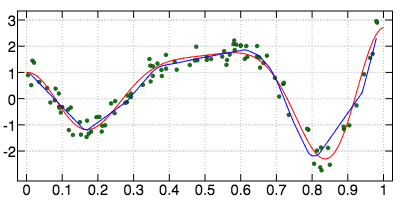
\includegraphics[width=\linewidth]{elm_1E_3}
\end{minipage}%
\hfill%
\begin{minipage}{0.4\textwidth}
\begin{verbatim}
   initelm 100
0
   elm 1E_3
\end{verbatim}
\end{minipage}
\vskip.5\baselineskip

\subsection{Test dataset}
A test set is used to assert the capacity of the model to generalize
on unseen data. Its size is fixed to $10\%$ of the size of the training set.

\nwenddocs{}\nwbegincode{29}\sublabel{NWS2xmL-15TB7-1}\nwmargintag{{\nwtagstyle{}\subpageref{NWS2xmL-15TB7-1}}}\moddef{testdat~{\nwtagstyle{}\subpageref{NWS2xmL-15TB7-1}}}\endmoddef\nwstartdeflinemarkup\nwusesondefline{\\{NWS2xmL-15el3j-1}}\nwenddeflinemarkup
XT=: ? (>. 0.1 * y) $ 0
YT=: f XT

\nwused{\\{NWS2xmL-15el3j-1}}\nwendcode{}\nwbegindocs{30}\nwdocspar
{\Tt{}test\nwendquote} computes the root mean square error (RMSE) on the test set.

\nwenddocs{}\nwbegincode{31}\sublabel{NWS2xmL-qrUr4-5}\nwmargintag{{\nwtagstyle{}\subpageref{NWS2xmL-qrUr4-5}}}\moddef{utils~{\nwtagstyle{}\subpageref{NWS2xmL-qrUr4-1}}}\plusendmoddef\nwstartdeflinemarkup\nwusesondefline{\\{NWS2xmL-2IxhEH-1}}\nwprevnextdefs{NWS2xmL-qrUr4-4}{\relax}\nwenddeflinemarkup
mean=: +/ % #
rmse=: [: %: [: mean ([: *: -)

\nwused{\\{NWS2xmL-2IxhEH-1}}\nwendcode{}\nwbegincode{32}\sublabel{NWS2xmL-Joiug-1}\nwmargintag{{\nwtagstyle{}\subpageref{NWS2xmL-Joiug-1}}}\moddef{test~{\nwtagstyle{}\subpageref{NWS2xmL-Joiug-1}}}\endmoddef\nwstartdeflinemarkup\nwusesondefline{\\{NWS2xmL-2IxhEH-1}}\nwenddeflinemarkup
test=: 3 : 0
  YThat=: (mkH ,. XT) mp c
  plottest 0
  YT rmse YThat
)

\nwused{\\{NWS2xmL-2IxhEH-1}}\nwendcode{}\nwbegincode{33}\sublabel{NWS2xmL-D6YgQ-1}\nwmargintag{{\nwtagstyle{}\subpageref{NWS2xmL-D6YgQ-1}}}\moddef{plottest~{\nwtagstyle{}\subpageref{NWS2xmL-D6YgQ-1}}}\endmoddef\nwstartdeflinemarkup\nwusesondefline{\\{NWS2xmL-2IxhEH-1}}\nwenddeflinemarkup
plottest=: 3 : 0
  \LA{}initplot~{\nwtagstyle{}\subpageref{NWS2xmL-1JSNQW-1}}\RA{}
  pd XT;YT
  pd 'color magenta'
  pd XT;YThat
  \LA{}plotf~{\nwtagstyle{}\subpageref{NWS2xmL-4gTINf-1}}\RA{}
  pd 'show'
)

\nwused{\\{NWS2xmL-2IxhEH-1}}\nwendcode{}\nwbegindocs{34}\nwdocspar
\noindent\begin{minipage}{0.5\textwidth}
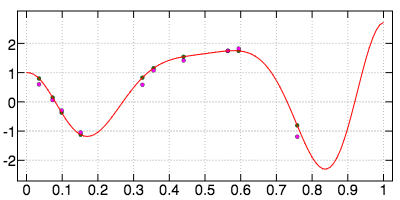
\includegraphics[width=\linewidth]{elmtest}
\end{minipage}%
\hfill%
\begin{minipage}{0.4\textwidth}
\begin{verbatim}
   test 0
0.172019
\end{verbatim}
\end{minipage}
\vskip.5\baselineskip

\nwenddocs{}\nwbegincode{35}\sublabel{NWS2xmL-3bJuaU-1}\nwmargintag{{\nwtagstyle{}\subpageref{NWS2xmL-3bJuaU-1}}}\moddef{require~{\nwtagstyle{}\subpageref{NWS2xmL-3bJuaU-1}}}\endmoddef\nwstartdeflinemarkup\nwusesondefline{\\{NWS2xmL-2IxhEH-1}}\nwenddeflinemarkup
require'trig'
require'plot'
require'numeric'

\nwused{\\{NWS2xmL-2IxhEH-1}}\nwendcode{}\nwbegincode{36}\sublabel{NWS2xmL-2IxhEH-1}\nwmargintag{{\nwtagstyle{}\subpageref{NWS2xmL-2IxhEH-1}}}\moddef{jelm.ijs~{\nwtagstyle{}\subpageref{NWS2xmL-2IxhEH-1}}}\endmoddef\nwstartdeflinemarkup\nwenddeflinemarkup
\LA{}require~{\nwtagstyle{}\subpageref{NWS2xmL-3bJuaU-1}}\RA{}
\LA{}utils~{\nwtagstyle{}\subpageref{NWS2xmL-qrUr4-1}}\RA{}
\LA{}dataset~{\nwtagstyle{}\subpageref{NWS2xmL-1BDS9S-1}}\RA{}
\LA{}plotdat~{\nwtagstyle{}\subpageref{NWS2xmL-MlnJE-1}}\RA{}
\LA{}plotpoly~{\nwtagstyle{}\subpageref{NWS2xmL-44Bx4d-1}}\RA{}
\LA{}polyreg~{\nwtagstyle{}\subpageref{NWS2xmL-16Ud8S-1}}\RA{}
\LA{}gram~{\nwtagstyle{}\subpageref{NWS2xmL-4YHogE-1}}\RA{}
\LA{}ridge~{\nwtagstyle{}\subpageref{NWS2xmL-Vqgr5-1}}\RA{}
\LA{}plotelm~{\nwtagstyle{}\subpageref{NWS2xmL-4OfyJI-1}}\RA{}
\LA{}elm~{\nwtagstyle{}\subpageref{NWS2xmL-3rGYkW-1}}\RA{}
\LA{}plottest~{\nwtagstyle{}\subpageref{NWS2xmL-D6YgQ-1}}\RA{}
\LA{}test~{\nwtagstyle{}\subpageref{NWS2xmL-Joiug-1}}\RA{}

\nwnotused{jelm.ijs}\nwendcode{}

\nwixlogsorted{c}{{dataset}{NWS2xmL-1BDS9S-1}{\nwixd{NWS2xmL-1BDS9S-1}\nwixu{NWS2xmL-2IxhEH-1}}}%
\nwixlogsorted{c}{{elm}{NWS2xmL-3rGYkW-1}{\nwixd{NWS2xmL-3rGYkW-1}\nwixd{NWS2xmL-3rGYkW-2}\nwixu{NWS2xmL-2IxhEH-1}}}%
\nwixlogsorted{c}{{gendat}{NWS2xmL-15el3j-1}{\nwixu{NWS2xmL-1BDS9S-1}\nwixd{NWS2xmL-15el3j-1}}}%
\nwixlogsorted{c}{{gram}{NWS2xmL-4YHogE-1}{\nwixd{NWS2xmL-4YHogE-1}\nwixd{NWS2xmL-4YHogE-2}\nwixu{NWS2xmL-2IxhEH-1}}}%
\nwixlogsorted{c}{{initplot}{NWS2xmL-1JSNQW-1}{\nwixu{NWS2xmL-MlnJE-1}\nwixd{NWS2xmL-1JSNQW-1}\nwixu{NWS2xmL-D6YgQ-1}}}%
\nwixlogsorted{c}{{jelm.ijs}{NWS2xmL-2IxhEH-1}{\nwixd{NWS2xmL-2IxhEH-1}}}%
\nwixlogsorted{c}{{noise}{NWS2xmL-148nWG-1}{\nwixu{NWS2xmL-1BDS9S-1}\nwixd{NWS2xmL-148nWG-1}}}%
\nwixlogsorted{c}{{plotdat}{NWS2xmL-MlnJE-1}{\nwixd{NWS2xmL-MlnJE-1}\nwixu{NWS2xmL-2IxhEH-1}}}%
\nwixlogsorted{c}{{plotelm}{NWS2xmL-4OfyJI-1}{\nwixd{NWS2xmL-4OfyJI-1}\nwixu{NWS2xmL-2IxhEH-1}}}%
\nwixlogsorted{c}{{plotf}{NWS2xmL-4gTINf-1}{\nwixu{NWS2xmL-MlnJE-1}\nwixd{NWS2xmL-4gTINf-1}\nwixu{NWS2xmL-D6YgQ-1}}}%
\nwixlogsorted{c}{{plotpoly}{NWS2xmL-44Bx4d-1}{\nwixd{NWS2xmL-44Bx4d-1}\nwixu{NWS2xmL-2IxhEH-1}}}%
\nwixlogsorted{c}{{plottest}{NWS2xmL-D6YgQ-1}{\nwixd{NWS2xmL-D6YgQ-1}\nwixu{NWS2xmL-2IxhEH-1}}}%
\nwixlogsorted{c}{{polyreg}{NWS2xmL-16Ud8S-1}{\nwixd{NWS2xmL-16Ud8S-1}\nwixu{NWS2xmL-2IxhEH-1}}}%
\nwixlogsorted{c}{{require}{NWS2xmL-3bJuaU-1}{\nwixd{NWS2xmL-3bJuaU-1}\nwixu{NWS2xmL-2IxhEH-1}}}%
\nwixlogsorted{c}{{ridge}{NWS2xmL-Vqgr5-1}{\nwixd{NWS2xmL-Vqgr5-1}\nwixu{NWS2xmL-2IxhEH-1}}}%
\nwixlogsorted{c}{{test}{NWS2xmL-Joiug-1}{\nwixd{NWS2xmL-Joiug-1}\nwixu{NWS2xmL-2IxhEH-1}}}%
\nwixlogsorted{c}{{testdat}{NWS2xmL-15TB7-1}{\nwixu{NWS2xmL-15el3j-1}\nwixd{NWS2xmL-15TB7-1}}}%
\nwixlogsorted{c}{{utils}{NWS2xmL-qrUr4-1}{\nwixd{NWS2xmL-qrUr4-1}\nwixd{NWS2xmL-qrUr4-2}\nwixd{NWS2xmL-qrUr4-3}\nwixd{NWS2xmL-qrUr4-4}\nwixd{NWS2xmL-qrUr4-5}\nwixu{NWS2xmL-2IxhEH-1}}}%
\nwbegindocs{37}\nwdocspar
\end{document}
\nwenddocs{}
